% chktex-file 44

\chapter{Methods}
\label{ch:methods}
This chapter presents the methodology of the proposed hybrid semantic exploration system, 
designed to mitigate the key limitations identified in Chapter~\ref{ch:sota}, namely the 
absence of persistent semantic memory, the reliance on single-source semantic detections, 
and the lack of an explicit and controllable trade-off between semantic exploration and 
exploitation in existing approaches.

The proposed system integrates zero-shot semantic perception with frontier-based exploration and persistent 3D semantic mapping into a unified, closed-loop decision-making framework. Semantic evidence acquired during exploration is continuously fused into a long-term spatial memory, while exploration behavior is adaptively modulated based on the reliability of accumulated semantic beliefs.

An overview of the system architecture is provided in Section~\ref{sec:methods:system_overview}, followed by detailed descriptions of the core components: semantic frontier exploration (Section~\ref{sec:methods:semantic_frontier}), promptable zero-shot detection (Section~\ref{sec:methods:zero_shot_detection}), persistent semantic 3D mapping (Section~\ref{sec:methods:persistent_mapping}), the multi-source fusion strategy governing semantic belief updates (Section~\ref{sec:methods:fusion_strategy}), and the behavior tree used to orchestrate semantic-guided exploration and navigation (Section~\ref{sec:methods:behavior_tree}).


\section{System Overview}
\label{sec:methods:system_overview}

The proposed system follows a modular hybrid architecture that tightly couples semantic perception,
geometry-driven exploration, and persistent semantic mapping to enable robust open-vocabulary
object-guided exploration. Figure~\ref{fig:system_overview} provides a high-level overview of the system components and their data flow. The exploration task is specified by a user-provided natural language prompt, which defines the semantic target and conditions the detection, exploration, and fusion modules throughout system execution.

\begin{figure}[h!]
    \centering
    \includegraphics[width=\textwidth]{Images/03_methods/sage_pipeline.png}
    \caption{Overview of the SAGE system architecture for open-vocabulary semantic exploration.
    RGB-D observations and robot poses are processed by three parallel modules: 
    (a) a persistent semantic mapping backend (OpenFusion~\cite{yamazakiOpenFusionRealtimeOpenVocabulary2023}) that maintains a semantic 3D map, 
    (b) a semantic frontier exploration module that scores geometric frontiers based on language-guided relevance, and 
    (c) a promptable zero-shot detection pipeline for object hypotheses.
    All semantic hypotheses are represented as graph nodes, filtered by relevance maps, and fused using a multi-source fusion strategy.
    A behavior tree orchestrates exploration, verification, and navigation actions, while low-level motion planning and execution are handled by the ROS~2 Navigation Stack~\cite{macenskiDesksROSMaintainers2023,makoviychukIsaacGymHigh2021}.}
\label{fig:system_overview}
\end{figure}

Robot observations at time $t$ are represented as RGB-D measurements $O_t = \{I_t, D_t\}$, where $I_t$ denotes the RGB image and $D_t$ the depth map. The robot pose in the world frame is denoted by $P_t$. To reduce computational load, observations are temporally and spatially downsampled prior to further processing.

The pre-processed observations are then fed into three parallel modules.
(a) The \textit{Memory Module} takes as input the current observations $O_t$ and pose $P_t$, obtained from the ROS~2 SLAM Toolbox~\cite{macenskiSLAMToolboxSLAM2021}, and updates the persistent semantic 3D map $M_t$.
(b) The \textit{Exploration Module} uses $O_t$ and $P_t$ to generate semantic frontiers $F_t$ from the current exploration occupancy grid.
(c) The \textit{Detection Module} processes $O_t$ to produce promptable zero-shot detections $D_t^{\text{det}}$.

Each module outputs a set of graph nodes representing semantic hypotheses.
Specifically, the memory module produces memory graph nodes $G_t^{\text{mem}}$ derived from the persistent map $M_t$, the exploration module outputs exploration graph nodes $G_t^{\text{exp}}$ corresponding to semantic frontiers $F_t$, and the detection module outputs detection graph nodes $G_t^{\text{det}}$ obtained from $D_t^{\text{det}}$.
This unified graph abstraction enables heterogeneous semantic hypotheses to be compared, filtered, and ranked using a common interface.

Prior to fusion, graph nodes are filtered using a relevance map to suppress nodes located in already explored areas. The remaining nodes are fused using the multi-source fusion strategy described in Section~\ref{sec:methods:fusion_strategy}, resulting in a unified set of weighted graph nodes $G_t^{\text{fused}}$.

Finally, the behavior tree described in Section~\ref{sec:methods:behavior_tree} selects the next high-level action based on $G_t^{\text{fused}}$, either navigating toward high-value frontiers for continued exploration or approaching detected objects for verification.
Low-level motion planning, obstacle avoidance, and execution are handled by the ROS~2 Navigation Stack~\cite{macenskiDesksROSMaintainers2023}.


\section{Semantic Frontier Exploration}
\label{sec:methods:semantic_frontier}

Semantic frontier exploration extends classical frontier-based exploration by incorporating
semantic relevance derived from vision-language models, enabling task-driven exploration guided by
a user-defined semantic prompt. Instead of exploring unknown space uniformly, the robot prioritizes frontiers that are more likely to yield observations relevant to the target concept~\cite{topiwalaFrontierBasedExploration2018, yamauchiFrontierbasedApproachAutonomous1997, yokoyamaVLFMVisionLanguageFrontier2023, alamaRayFrontsOpenSetSemantic2025}. Figure~\ref{fig:sage_maps} illustrates the intermediate map representations and processing stages used to construct the semantic frontier map.

\subsection*{Exploration Occupancy Maps}

The system maintains three distinct 2D occupancy grids for navigation and exploration:
(a) a SLAM map used for localization and navigation~\cite{macenskiSLAMToolboxSLAM2021},
(b) an exploration map used exclusively for frontier detection, and
(c) an inflated map that suppresses narrow passages and noisy frontier artifacts.
This separation decouples stable navigation from task-specific exploration decisions and prevents
semantic exploration logic from modifying the navigation map.

\begin{figure}[h!]
    \centering
    \includegraphics[width=\textwidth]{Images/03_methods/semantic_frontier_exploration/sage_maps.png}
    \caption{Overview of the map representations used for semantic frontier exploration.
    The SLAM map is used for localization and navigation, while the exploration map encodes
    task-specific explored and unexplored regions for frontier detection~\cite{macenskiSLAMToolboxSLAM2021}.
    An inflated map is used to suppress narrow structures and reduce spurious frontiers.
    The resulting frontier map is combined with a semantic value map to prioritize exploration
    toward semantically relevant regions.}
    \label{fig:sage_maps}
\end{figure}

Rather than running a separate SLAM instance for exploration, the exploration map is derived
directly from the SLAM occupancy grid~\cite{macenskiSLAMToolboxSLAM2021}.
Given the robot pose $P_t$ and the SLAM map $M_{\text{SLAM}}$, free space is raycast from the robot
into the occupancy grid, using the known sensor model and maximum sensor range, marking traversed cells as explored while preserving unknown regions beyond sensor reach. This raycasting process is applied to all recorded robot poses accumulated during the current task, yielding an exploration map $M_{\text{exp}}$ that reflects the explored workspace.

When a new semantic search task is initiated, all stored poses are cleared and the exploration map
is rebuilt from scratch, while the SLAM map remains unchanged.
This design ensures that exploration decisions are conditioned solely on task-relevant semantic
information and prevents bias from previously explored but semantically irrelevant regions.

\subsection*{Frontier Detection and Calculation}

Frontiers are defined as the boundary between known free space and unknown regions in the exploration occupancy grid~\cite{topiwalaFrontierBasedExploration2018} (see Figure~\ref{fig:frontier_detection}). This work uses the algorithm outlined in Algorithm~\ref{alg:extract_frontiers} to extract and cluster frontiers from the exploration map. 

\begin{figure}[h!]
    \centering
    \includegraphics[width=\textwidth]{Images/03_methods/frontier_example.png}
    \caption{Example of frontier detection on the exploration occupancy grid.
    Frontiers are identified as free cells adjacent to unknown space and clustered into spatially
    contiguous regions, with centroids serving as candidate exploration targets.}
    \label{fig:frontier_detection}
\end{figure}

Let $\mathcal{G} \in \{-1, 0, 100\}^{W \times H}$ denote the exploration occupancy grid, where $-1$ represents unknown space, $0$ free space, and $100$ occupied space~\cite{macenskiSLAMToolboxSLAM2021}. The set $\mathcal{F}_t$ denotes the set of detected frontier clusters at time step $t$. Each frontier cluster $\mathcal{P}$ is a set of spatially connected frontier cells. The set $\{\mathbf{c}_i^{t-1}\}$ contains the centroids of frontier clusters detected at the previous time step and is used to maintain temporal consistency via centroid matching.

\begin{algorithm}[H]
\caption{Geometric frontier extraction and clustering from the exploration occupancy grid}\label{alg:extract_frontiers}
\begin{algorithmic}[1]

\Function{ExtractFrontiers}{
    $\mathcal{G}$,
    $N_{\min}$,
    $N_{\max}$,
    $d_{\text{match}}$,
    $\{\mathbf{c}_{i}^{t-1}\}$
}
    \State $\mathcal{F}_t \gets \emptyset$ \Comment{Output set of clustered frontiers}

    \ForAll{cells $(x,y)$ with $\mathcal{G}(x,y)=0$} \Comment{Iterate over free cells}
        \If{$\mathcal{G}(x,y)=0$ \textbf{and} any 4-neighbor is unknown}
            \State Mark $(x,y)$ as frontier \Comment{Free–unknown boundary}
        \EndIf
    \EndFor

    \ForAll{unvisited frontier cells $(x,y)$}
        \State Grow a cluster $\mathcal{P}$ using 8-connected BFS
        \Comment{Spatially connected frontier region}

        \If{$N_{\min} \le |\mathcal{P}| \le N_{\max}$}
            \State Compute centroid $\mathbf{c} \gets \frac{1}{|\mathcal{P}|} \sum_{\mathbf{p} \in \mathcal{P}} \mathbf{p}$
            \Comment{Representative frontier location}

            \State Assign frontier ID via nearest centroid match within $d_{\text{match}} \in \mathbb{R}$

            \If{no match found}
                \State Assign new frontier ID \Comment{Newly discovered frontier}
            \EndIf

            \State Add $(\mathcal{P}, \mathbf{c})$ to $\mathcal{F}_t$
            \Comment{Store valid frontier}
        \EndIf
    \EndFor

    \State \Return $\mathcal{F}_t$ \Comment{Set of clustered, tracked frontiers}
\EndFunction

\end{algorithmic}
\end{algorithm}

The extracted frontier cells are clustered using an 8-connected \ac{BFS} to group spatially contiguous regions. Clusters that fall within predefined size limits ($N_{\min}$ and $N_{\max}$) are retained, while outliers are discarded.
Each valid frontier cluster is represented by its centroid, which serves as the candidate exploration target. Let $\mathcal{P} = \{\mathbf{p}_j \in \mathbb{R}^2 \mid j = 1,\dots,|\mathcal{P}|\}$ denote the set of grid cell coordinates belonging to a frontier cluster. The centroid $\mathbf{c} \in \mathbb{R}^2$ is defined as the arithmetic mean of the spatial coordinates of all cells belonging to the frontier cluster. Frontier identity matching is performed using nearest-neighbor association in Euclidean space, where a frontier centroid is assigned the ID of the closest previously observed centroid within distance $d_{\text{match}} \in \mathbb{R}$, otherwise a new frontier ID is created.

\begin{equation}
\label{eq:frontier_centroid}
\mathbf{c} = \frac{1}{|\mathcal{P}|} \sum_{\mathbf{p} \in \mathcal{P}} \mathbf{p}
\end{equation}

Equation~\ref{eq:frontier_centroid} yields a single representative location that approximates the geometric center of the frontier region. This centroid is used as the navigation target for frontier-based exploration and as the reference position for semantic
scoring.

The frontier centroids are tracked over time by matching them to previously detected frontiers based on spatial proximity, allowing for consistent identification of persistent frontiers across time steps. To extract the semantically most relevant frontiers, each frontier is scored using the value map generated by the \ac{VLM} as described below~\cite{yokoyamaVLFMVisionLanguageFrontier2023}. The scoring procedure is outlined in Algorithm~\ref{alg:value_map_query} and Algorithm~\ref{alg:semantic_frontier_update}. Let $\mathcal{C} = \{(x_i, y_i, s_i)\}$ denote the semantic value map represented as a set of 2D cells with associated semantic scores $s_i$, obtained by temporally aggregating cosine similarity values between vision-language model embeddings and the user-defined text prompt (Section~\ref{sec:semantic_frontier:value_map_generation}). For a value map cell $q \in \mathcal{C}$, $s(q)$ denotes the semantic similarity score stored at that cell.

\begin{algorithm}[H]
\caption{Value Map Mask for scoring Frontiers}
\label{alg:value_map_query}
\begin{algorithmic}[1]

\Function{GetScoreFromValueMap}{
    $\mathcal{C}$,
    $\mathbf{p}$
}
    \State $r \gets 0.3$ \Comment{Query radius}
    \State $s_{\max} \gets 0$
    \State $\text{observed} \gets \text{false}$
    
    \ForAll{points $q \in \mathcal{C}$}
        \If{$\lVert q - \mathbf{p} \rVert_2 < r$}
            \State $s_{\max} \gets \max(s_{\max}, s(q))$
            \Comment{Max semantic response}
            \State $\text{observed} \gets \text{true}$
        \EndIf
    \EndFor

    \If{$\text{observed}$}
        \State \Return $(\text{observed}=\text{true},\; \text{score}=s_{\max})$
    \Else
        \State \Return $(\text{observed}=\text{false})$
    \EndIf

\EndFunction

\end{algorithmic}
\end{algorithm}


The value map is a 2D grid in which each cell stores temporally aggregated cosine similarity scores
(see Section~\ref{sec:semantic_frontier:value_map_generation}) between \ac{VLM}
embeddings of scene observations and a user-defined text prompt.
Let $\mathcal{V} = \{(x_i, y_i, s_i)\}$ denote the value map, where $(x_i, y_i)$ are grid coordinates
and $s_i \in \mathbb{R}$ is the associated semantic similarity score.

To score a frontier, its centroid $\mathbf{c} \in \mathbb{R}^2$ is projected into the value map
coordinate frame.
The semantic score of the frontier is obtained by querying the maximum similarity score within a
fixed-radius neighborhood around $\mathbf{c}$, as described in
Algorithm~\ref{alg:value_map_query}.
If no valid score exists within this neighborhood, indicating that the region has not yet been
observed, the frontier is marked as unobserved.
Using the maximum response emphasizes strong semantic evidence while remaining robust to noise and
partial observations, consistent with prior semantic frontier scoring approaches~\cite{yokoyamaVLFMVisionLanguageFrontier2023}.

Algorithm~\ref{alg:semantic_frontier_update} summarizes the construction of semantic frontier graph
nodes by combining geometric frontier extraction with semantic scoring.

\begin{algorithm}[H]
\caption{Construction of semantic frontier graph nodes}
\label{alg:semantic_frontier_update}
\begin{algorithmic}[1]

\Function{UpdateSemanticFrontiers}{
    $\mathcal{G}$,
    $\mathcal{V}$,
    $\{\mathbf{c}_{i}^{t-1}\}$
}
    \State $\mathcal{F}_t \gets \textsc{ExtractFrontiers}(\mathcal{G}, N_{\min}, N_{\max}, d_{\text{match}}, \{\mathbf{c}_{i}^{t-1}\})$
    \Comment{Geometric frontier extraction}

    \ForAll{frontier $f \in \mathcal{F}_t$}
        \State $\mathbf{c} \gets \text{centroid}(f)$
        \Comment{Representative frontier position}

        \State $(\text{observed}, s) \gets \textsc{GetScoreFromValueMap}(\mathcal{V}, \mathbf{c})$
        \Comment{Semantic value lookup}

        \State Create graph node $n$
        \State $n.\text{id} \gets f.\text{id}$
        \State $n.\text{position} \gets \mathbf{c}$
        \State $n.\text{score} \gets s$
        \State $n.\text{observed} \gets \text{observed}$

        \State Add $n$ to graph
        \Comment{Semantic frontier node}
    \EndFor

    \State Publish frontier graph
    \Comment{For downstream task and visualization}

\EndFunction

\end{algorithmic}
\end{algorithm}

The final step involves creating graph nodes for each frontier, encapsulating their ID, position, semantic score, and observation status. These semantic frontier graph nodes form the primary input to the fusion strategy and behavior tree described in Sections~\ref{sec:methods:fusion_strategy} and~\ref{sec:methods:behavior_tree}.

\section*{Value Map Generation using Vision-Language Models}
\label{sec:semantic_frontier:value_map_generation}

The value map can be interpreted as an analogy to gradient ascent in deep reinforcement learning, where the robot seeks to maximize an expected semantic reward by navigating toward regions with high relevance to a target concept~\cite{yokoyamaVLFMVisionLanguageFrontier2023,gadreCoWsPastureBaselines2022,majumdarZSONZeroShotObjectGoal2023,thomasPolicyGradientMethods2017}. In this work, the value map represents the slope of a semantic reward function. In contrast to classical gradient ascent, movement toward regions of high semantic relevance is constrained by obstacles and unknown space. Consequently, geometrically derived frontiers serve as feasible navigation targets that guide the robot toward high-value regions while ensuring safe traversal, thereby preventing convergence to unreachable local maxima~\cite{gadreCoWsPastureBaselines2022}. Figure~\ref{fig:methods:gradient_ascent} illustrates this analogy, showing the semantic reward landscape and the role of frontier-based navigation (see Chapter~\ref{sec:methods:fusion_strategy} for the reward definition).

\begin{figure}[h!]
    \centering
    \includegraphics[width=\textwidth]{Images/03_methods/semantic_frontier_exploration/gardient_ascent.png}
    \caption{Conceptual visualization of the gradient-ascent analogy for semantic frontier exploration. Semantic relevance is illustrated as a folded reward surface, where frontier and memory graph nodes are elevated according to their semantic scores at position $(x,y)$.
    Geometric frontiers constrain feasible ascent directions under spatial obstacles.}
    \label{fig:methods:gradient_ascent}
\end{figure}

The value map is generated using a pre-trained vision-language model, specifically BLIP-2~\cite{liBLIP2BootstrappingLanguageImage2023}, which is queried via a ROS~2 service to compute semantic similarity between visual observations and a user-defined text prompt.
The value map node subscribes to RGB images, robot poses, and a global occupancy grid produced by a
LiDAR-based SLAM system. This differs from prior semantic frontier approaches such as VLFM~\cite{yokoyamaVLFMVisionLanguageFrontier2023}, which rely on depth camera projections and odometry-based local maps. By leveraging LiDAR-based SLAM, the proposed system maintains a globally consistent exploration map with reduced drift, enabling persistent semantic value accumulation over long trajectories. Figure~\ref{fig:methods:value_map_ros2_pipeline} illustrates the overall value map generation pipeline.

\begin{figure}[h!]
    \centering
    \includegraphics[width=\textwidth]{Images/03_methods/semantic_frontier_exploration/value_map_ros2_pipeline.png}
    \caption{ROS~2 value map generation pipeline using the BLIP-2 vision-language model for computing image-text cosine similarity.}
    \label{fig:methods:value_map_ros2_pipeline}
\end{figure}

Upon receiving an RGB image and a text prompt, the BLIP-2 service computes an image embedding and a text embedding using its pre-trained visual and textual encoders. The input image is divided into a grid of fixed-size patches, which are flattened, added with positional embeddings, and linearly projected before being processed by a vision transformer to capture spatial and semantic context~\cite{sharirImageWorth16x162021,liBLIP2BootstrappingLanguageImage2023}. Similarly, the text prompt is tokenized into subword units, embedded, and processed by a language transformer to model semantic and syntactic relationships.

Therefore, both embeddings are projected using learned projection matrices \( W_I \) and \( W_T \)
into a common embedding space (see Equation~\ref{eq:methods:value_map:projection}):

\begin{equation}
E_I = W_I f_I(I), \qquad
E_T = W_T f_T(T)
\label{eq:methods:value_map:projection}
\end{equation}

where \( f_I(\cdot) \) and \( f_T(\cdot) \) denote the visual and textual encoders, respectively.
The projection matrices \( W_I \) and \( W_T \) are learned during pre-training using an
\ac{ITC} objective, which optimizes the cosine similarity between matching
image-text pairs while pushing apart non-matching pairs~\cite{radfordLearningTransferableVisual2021,liBLIP2BootstrappingLanguageImage2023}. This training procedure aligns visual and textual representations in a shared semantic embedding space, enabling direct similarity comparison via cosine similarity. The projected embeddings are subsequently L2-normalized to unit length, which is required for cosine similarity computation.

The cosine similarity score \( S \) between the normalized image embedding \( \hat{E}_I \) and text embedding \( \hat{E}_T \) is computed as:

\begin{equation}
S = \hat{E}_I \cdot \hat{E}_T
  = \frac{E_I}{\|E_I\|_2} \cdot \frac{E_T}{\|E_T\|_2} = \cos(\hat{E}_I, \hat{E}_T)
\label{eq:methods:value_map:cosine_similarity}
\end{equation}

Figure~\ref{fig:methods:cosine_sim} illustrates this image-text similarity computation, where
visual observations are embedded by the BLIP-2 image encoder and compared against a
user-defined text prompt in a shared semantic embedding space. Although cosine similarity is theoretically bounded in the interval \([-1,1]\), in practice \ac{ITC}-based \acp{VLM} yield similarity scores concentrated in a narrow positive range~\cite{radfordLearningTransferableVisual2021,liBLIP2BootstrappingLanguageImage2023}. This continuous score serves as a measure of semantic relevance between the current visual observation and the target concept.

\begin{figure}[h!]
    \centering
    \includegraphics[width=\textwidth]{Images/03_methods/blip2_cosine_sim.png}
    \caption{Image-text cosine similarity computation using the BLIP-2 \ac{ITC} head.
    An RGB observation is embedded by the visual encoder and compared against a user-defined text prompt in a shared semantic embedding space~\cite{liBLIP2BootstrappingLanguageImage2023}.}
    \label{fig:methods:cosine_sim}
\end{figure}

\subsubsection*{Cosine Similarity to Value Map Projection}

The computed cosine similarity score is integrated into a persistent 2D semantic value map in a
pose- and visibility-aware manner.
Let $V_{t-1}$ denote the semantic value map and $C_{t-1}$ the associated confidence map at time
step $t-1$, and let $s_t$ be the cosine similarity score obtained from the \ac{VLM}
at the current robot pose $\mathbf{p}_t$.

The update procedure, summarized in Algorithm~\ref{alg:value_map_update}, consists of three
conceptual stages: (a) motion-gated temporal decay, (b) visibility-aware observation selection, and
(c) confidence-weighted fusion. The following update procedure closely follows the semantic value map formulation proposed in VLFM~\cite{yokoyamaVLFMVisionLanguageFrontier2023}, with adaptations for ROS~2 integration.

\begin{algorithm}[H]
\caption{2D Value Map Update using Vision-Language Model Similarity Scores}
\label{alg:value_map_update}
\begin{algorithmic}[1]

\Function{UpdateSemanticValueMap}{
    $V_{t-1}$,
    $C_{t-1}$,
    $s_t$,
    $\mathbf{p}_t$
}

    \State \algcomment{(a) Motion-gated temporal decay}
    \If{$\|\mathbf{p}_t - \mathbf{p}_{t-1}\|_2 > \delta_{\text{move}}$}
        \State $V_{t-1} \gets \lambda V_{t-1}$
        \State $C_{t-1} \gets \lambda C_{t-1}$
    \EndIf

    \State \algcomment{(b) Visibility and observation confidence}
    \State Compute visibility mask $M_{\text{fov}}(\mathbf{p}_t)$ via raytracing
    \State Compute confidence map $C_{\text{obs}}(\mathbf{p}_t, M_{\text{fov}})$

    \State \algcomment{(c) Confidence-weighted fusion}
    \ForAll{cells $(i,j)$ with $M_{\text{fov}}(i,j)=1$}

        \State $v \gets V_{t-1}(i,j)$
        \State $c \gets C_{t-1}(i,j)$
        \State $c_{\text{new}} \gets C_{\text{obs}}(i,j)$

        \If{$c + c_{\text{new}} = 0$}
            \State \textbf{continue}
        \EndIf

        \State $V_t(i,j) \gets v + \alpha\, c_{\text{new}} (s_t - v)$
        \State $C_t(i,j) \gets \max(\lambda c,\; c_{\text{new}})$

    \EndFor

    \State \Return $V_t,\; C_t$
\EndFunction
\end{algorithmic}
\end{algorithm}

(a) Temporal decay is applied to both the value map and the confidence map only if the robot
has translated more than a predefined threshold $\delta_{\text{move}}$ since the previous update.
This motion-gated decay prevents repeated observations from dominating the map when the robot
remains stationary or performs pure rotations, while still allowing outdated semantic evidence
to fade over time when the robot explores new regions. The decay factor
$\lambda \in [0,1]$ controls the persistence of past observations and prevents oscillation between multiple similar frontiers by gradually reducing the influence of stale semantic evidence when the robot revisits similar viewpoints~\cite{yokoyamaVLFMVisionLanguageFrontier2023}.

(b) The set of map cells that can be updated at time step $t$ is determined by computing a
top-down visibility mask $M_{\text{fov}}(\mathbf{p}_t)$ using raytracing within the current field
of view, instead of relying solely on depth camera projections based on odometry~\cite{yokoyamaVLFMVisionLanguageFrontier2023,thrunProbabilisticRobotics2006}. Only cells that are geometrically visible from the robot's pose and not occluded by obstacles are considered for update. For these visible cells, an instantaneous observation confidence map $C_{\text{obs}}(\mathbf{p}_t, M_{\text{fov}})$ is computed, which models the reliability of the current observation as a function of the sensor geometry. Cells near the center of the field of view are assigned higher confidence, while confidence decreases toward the periphery due to reduced resolution and increased distortion. This behavior is modeled using a Gaussian weighting function over the angular deviation from the camera’s principal viewing direction. The observation confidence assigned to a visible cell $(i,j)$ is computed as

\begin{equation}
\label{eq:value_map:confidence_weight}
C_{\text{obs}}(i,j)
=
\mathrm{e}^{-\frac{1}{2}
\left(
\frac{\Delta\theta(i,j)}{\sigma}
\right)^2},
\end{equation}

where $\Delta\theta(i,j)$ denotes the angular difference between the viewing ray toward cell
$(i,j)$ and the robot’s forward-facing direction, and $\sigma$ controls the sharpness of the
confidence decay within the field of view. Smaller values of $\sigma$ result in a narrower high-confidence region centered around the optical axis, while larger values produce a more uniform confidence distribution. This confidence formulation follows the angular weighting strategy used in VLFM to model observation reliability across the field of view~\cite{yokoyamaVLFMVisionLanguageFrontier2023}.


(c) For each visible cell $(i,j)$, the semantic value stored in the map is updated toward the
current similarity score $s_t$ using a confidence-weighted fusion rule.
Let $V_{t-1}(i,j)$ and $C_{t-1}(i,j)$ denote the semantic value and confidence stored at cell $(i,j)$
before the update, and let $C_{\text{obs}}(i,j)$ denote the instantaneous observation confidence
computed from the current field of view.

The semantic value update is formulated as a weighted interpolation between the previous value and
the current similarity score (see Equation~\eqref{eq:value_map:update}):

\begin{equation}
\label{eq:value_map:update}
V_t(i,j)
=
V_{t-1}(i,j)
+
\alpha\, C_{\text{obs}}(i,j)
\bigl(
s_t - V_{t-1}(i,j)
\bigr),
\end{equation}

where $\alpha \in [0,1]$ is an update gain that controls how strongly new observations influence the
existing value map. Higher observation confidence leads to a stronger correction toward the current similarity score, while low-confidence observations have only a minor effect. In parallel, the confidence map is updated to preserve strong observations over time. Specifically, the confidence assigned to each cell is defined in Equation~\eqref{eq:value_map:confidence_update}:

\begin{equation}
\label{eq:value_map:confidence_update}
C_t(i,j)
=
\max\!\bigl(
\lambda\, C_{t-1}(i,j),
\;
C_{\text{obs}}(i,j)
\bigr),
\end{equation}

where $\lambda \in [0,1]$ is the temporal decay factor applied when the robot has translated since
the previous update. Using a max operation ensures that regions which have been observed with high confidence remain influential even after decay, preventing repeated low-confidence observations from diluting reliable semantic evidence~\cite{yokoyamaVLFMVisionLanguageFrontier2023}.

Together, Equations~\eqref{eq:value_map:update} and~\eqref{eq:value_map:confidence_update} implement
a persistent, confidence-aware fusion mechanism that incrementally integrates semantic similarity
scores into a spatially consistent value map.

Figure~\ref{fig:methods:value_map:example} illustrates a generated value map for the prompts ``Bed'', ``TV'', and the zero-shot prompt ``A door leading to a bed'', demonstrating how prompt design can bias exploration toward multiple targets or semantically useful transition regions.


\begin{figure}[h!]
    \centering
    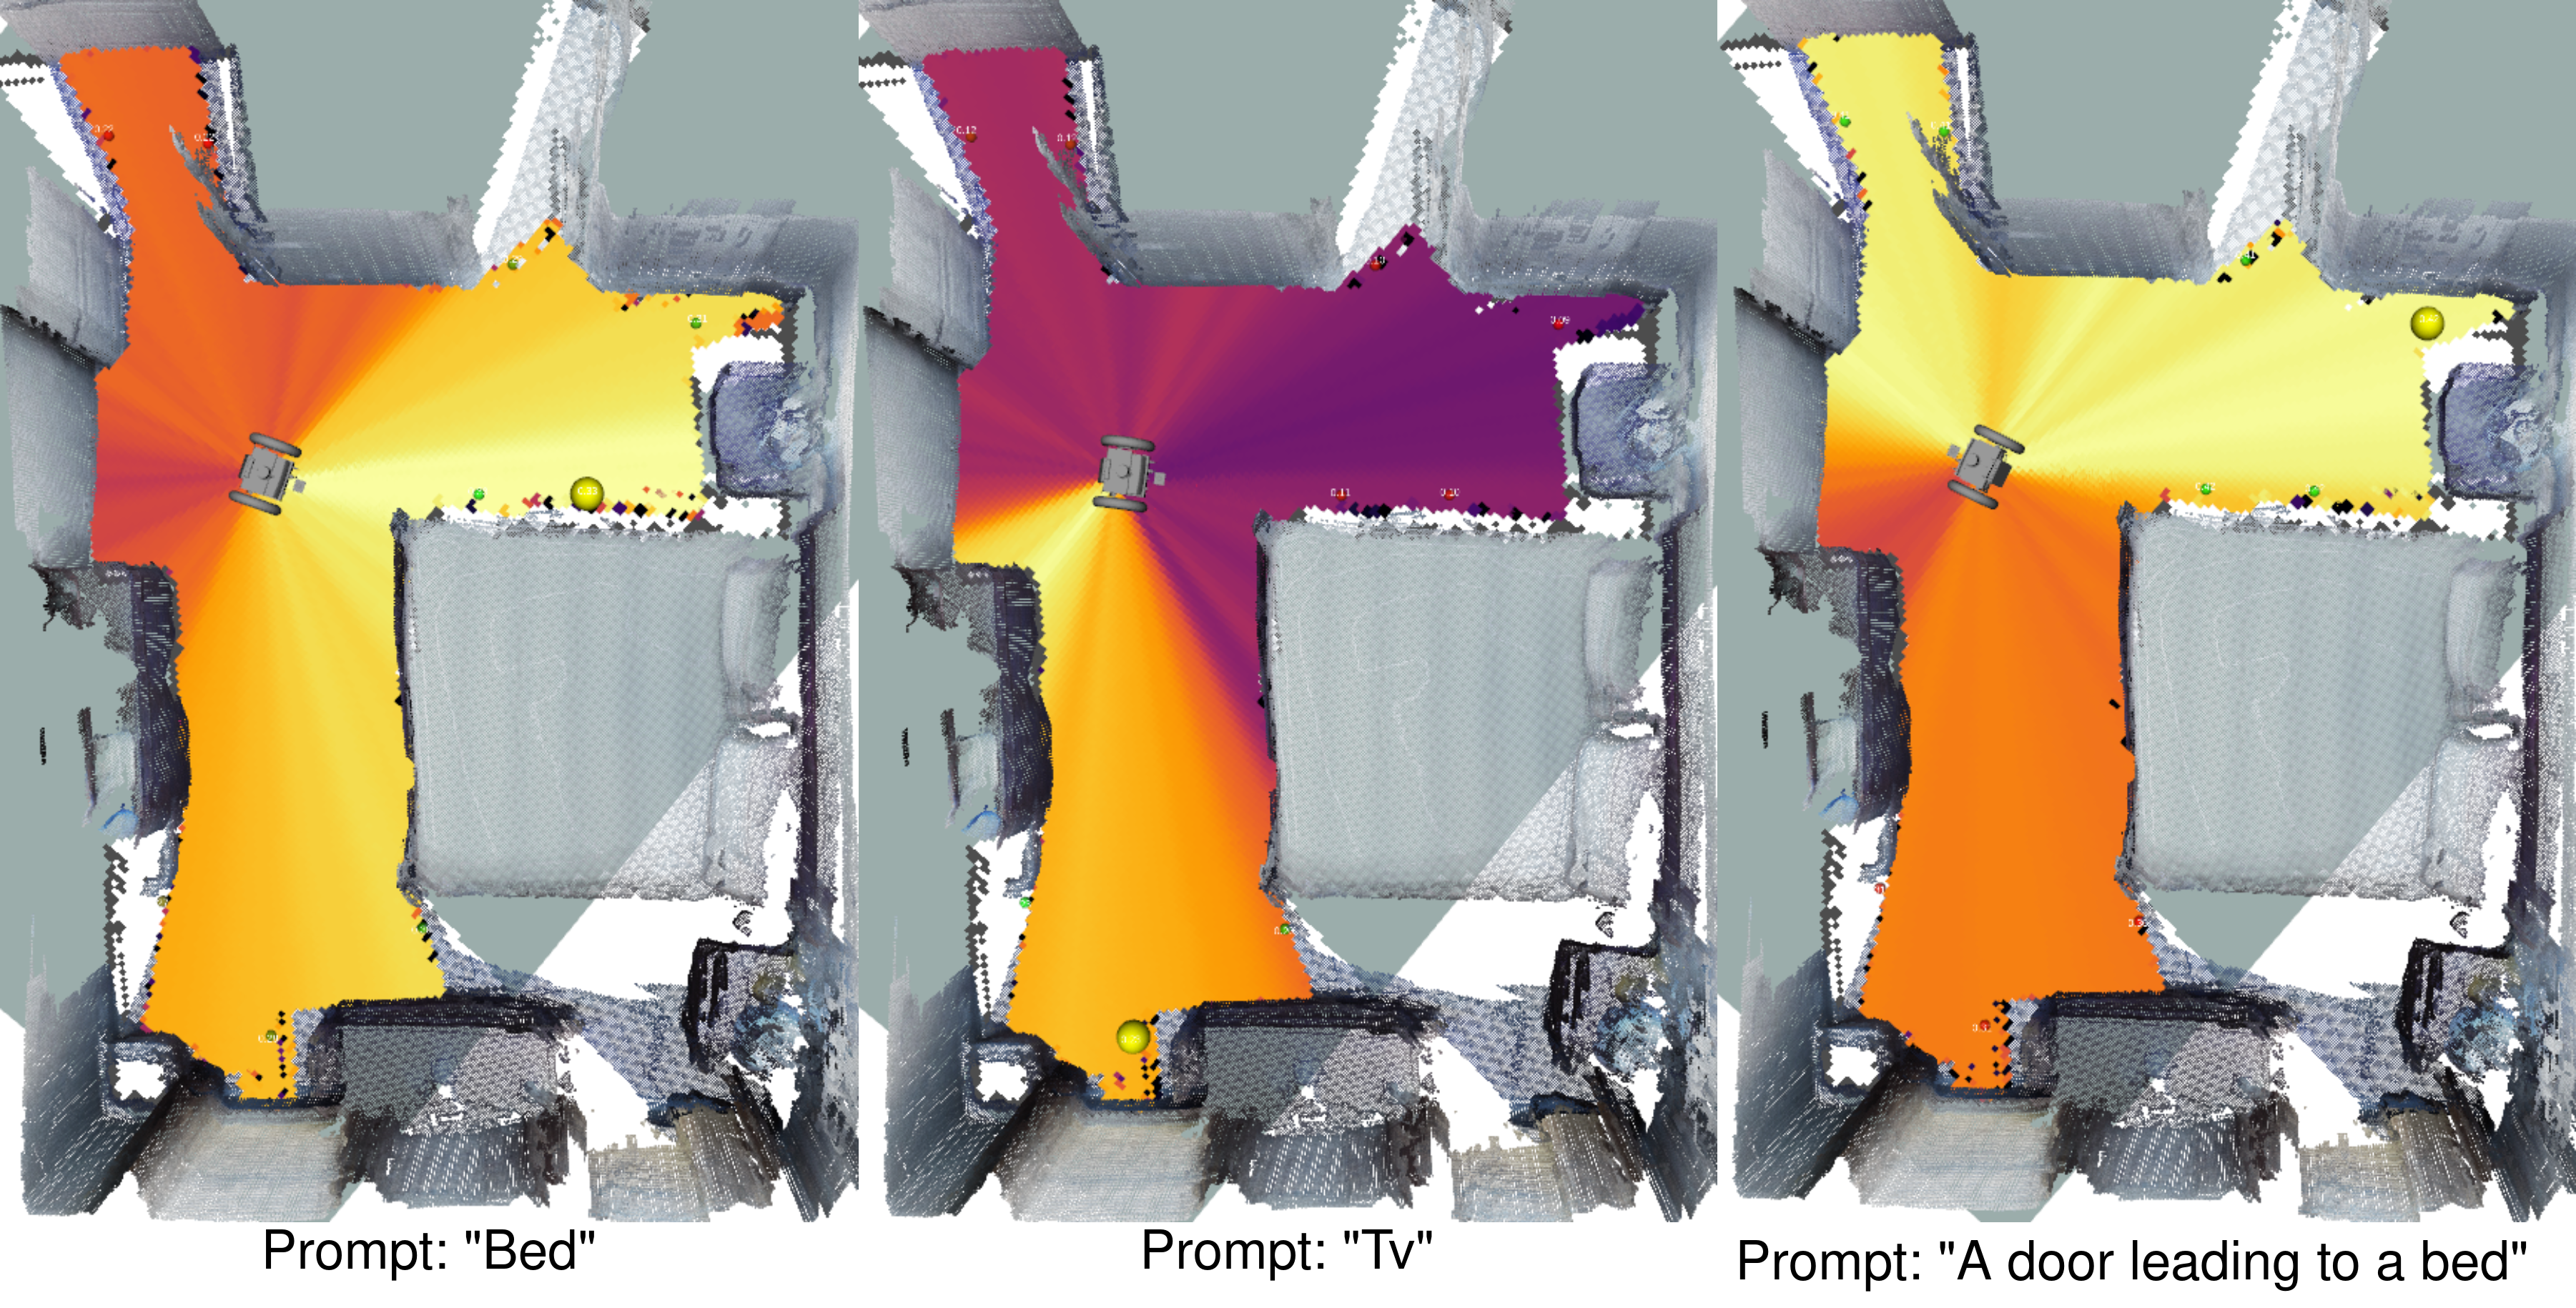
\includegraphics[width=\textwidth]{Images/03_methods/value_map_example.png}
    \caption{Example value maps generated using BLIP-2 for different text prompts.
    The value maps highlight regions of high semantic relevance to the prompts ``Bed'', ``TV'', and ``A door leading to a bed''.}
    \label{fig:methods:value_map:example}
\end{figure}

These scored frontiers are then encapsulated as graph nodes and passed to the fusion strategy
(Section~\ref{sec:methods:fusion_strategy}) for integration with memory and detection modules.

\section{Persistent Semantic 3D Mapping}
\label{sec:methods:persistent_mapping}


The semantic frontier centroids described in Section~\ref{sec:methods:semantic_frontier} offer
short-term exploration targets based on immediate observations. However, to enable effective multi-object search over multiple objects, the system requires a persistent memory that retains information about previously observed objects and their spatial locations throughout the exploration task~\cite{jiangDualMapOnlineOpenVocabulary2025,guConceptGraphsOpenVocabulary3D2023,buschOneMapFind2025}. The proposed system incorporates a semantic 3D mapping module that constructs a global, persistent semantic representation from RGB-D observations and produces object-level hypotheses in the form of graph nodes. These memory graph nodes are subsequently integrated into the fusion strategy (see Section~\ref{sec:methods:fusion_strategy}) to inform exploration and detection decisions.

At the time of implementation, OpenFusion~\cite{yamazakiOpenFusionRealtimeOpenVocabulary2023}
represented a suitable open-source framework for real-time, open-vocabulary semantic 3D mapping. Its balance between reconstruction fidelity and computational efficiency makes it suitable for onboard deployment on mobile robotic platforms~\cite{yamazakiOpenFusionRealtimeOpenVocabulary2023}. As discussed in the state-of-the-art analysis
(Chapter~\ref{sec:sota:semantic_scene_reconstruction}), OpenFusion enables zero-shot semantic
mapping but does not provide an object-centric abstraction. This work extends OpenFusion with
object-level semantic clustering and graph node generation, yielding a persistent semantic
memory tailored to multi-object search and long-horizon exploration tasks.

\subsection*{Global Map Construction with OpenFusion}

OpenFusion~\cite{yamazakiOpenFusionRealtimeOpenVocabulary2023} was originally designed for offline semantic reconstruction from pre-recorded
RGB-D sequences, such as ScanNet~\cite{daiScanNetRichlyannotated3D2017} and
Replica~\cite{straubReplicaDatasetDigital2019}. In contrast, this work adapts OpenFusion for
online operation on a mobile robot by integrating it with a LiDAR-based SLAM system that
provides globally consistent pose estimates.

A dedicated ROS~2 wrapper node, referred to as \texttt{openfusion\_ros}, interfaces OpenFusion
with the exploration system (see Figure~\ref{fig:methods:persistent_mapping:pipeline}). 

\begin{figure}[h!]
    \centering
    \includegraphics[width=\textwidth]{Images/03_methods/semantic_mapping/openfusion_ros_pipeline.png}
    \caption{ROS~2 integration of OpenFusion for persistent semantic 3D mapping.
    RGB images, depth images, and LiDAR-based SLAM poses are synchronized and filtered before
    integration into a global TSDF volume.
    On-demand semantic queries generate semantic and panoptic point clouds, which are further
    processed to extract object-level hypotheses for the fusion strategy.}
    \label{fig:methods:persistent_mapping:pipeline}
\end{figure}

The wrapper subscribes to RGB images $I_t$, depth images $D_t$, camera intrinsics $K$, and SLAM-based robot poses $P_t$. To limit computational overhead and avoid redundant observations, RGB-D ($I_t, D_t$) frames are forwarded to OpenFusion only if the robot pose $P_t$ differs sufficiently from previously integrated viewpoints. This pose filtering reduces redundant TSDF updates from near-identical viewpoints, mitigates over-integration artifacts, and ensures efficient use of the fixed voxel budget. Specifically, an input tuple \(\{(I_t, D_t, P_t)\}\) is accepted only if the robot has translated or rotated more than a predefined threshold \(\delta_{\text{move}}\) and represents a novel viewpoint relative to the existing map.

Upon initialization, OpenFusion is configured using the current camera intrinsics and a fixed
voxel resolution and voxel budget, which together define the available memory for semantic
mapping~\cite{yamazakiOpenFusionRealtimeOpenVocabulary2023}. For each accepted RGB-D observation \((I_t, D_t, P_t)\), the data are fused into a global \ac{TSDF} volume using the SLAM-based pose estimate, yielding a globally consistent 3D reconstruction with reduced drift compared to odometry-only approaches~\cite{thrunProbabilisticRobotics2006}.

Each point in the semantic point cloud is associated with a cosine similarity score between the
user-defined text prompt and the corresponding visual observation.
The visual embeddings are obtained using \ac{SEEM}~\cite{zouSegmentEverythingEverywhere2023}, a pre-trained \ac{VLM} optimized for dense, pixel-level representations. SEEM produces a high-dimensional embedding for each pixel in the RGB image, which is then compared
to the text prompt embedding using cosine similarity. By projecting these pixel-wise similarity scores into 3D space via the aligned RGB-D observations, a semantic point cloud is obtained in which each point encodes its semantic relevance with respect to the query.

% To enable object-level reasoning, SEEM~\cite{zouSegmentEverythingEverywhere2023} produces dense, pixel-level semantic predictions and associated similarity scores with respect to the query prompt.
In practice, only the most semantically relevant predictions are retained by selecting a subset
of high-confidence regions, controlled by a top-$k$ selection criterion. This selection acts as a filtering mechanism rather than a strict object count, limiting the number of candidate regions considered for further processing.

Based on these high-confidence regions, SEEM performs instance-aware grouping, yielding a
panoptic point cloud in which each 3D point is assigned both a semantic label and an instance
identifier~\cite{zouSegmentEverythingEverywhere2023}.
This panoptic representation allows spatially distinct object instances of the same semantic
class to be differentiated. While OpenFusion provides the underlying 3D reconstruction and voxel management, semantic embeddings are computed externally using SEEM and fused into the 3D map via aligned RGB-D projections~\cite{zouSegmentEverythingEverywhere2023,yamazakiOpenFusionRealtimeOpenVocabulary2023}.

These instance-level clusters are subsequently aggregated into object-centric
memory graph nodes, which are consumed by the fusion strategy for long-horizon
semantic exploration and object search.


\subsection*{Semantic Clustering and Graph Node Generation}

The semantic point cloud produced by OpenFusion encodes dense geometric structure together
with a per-point semantic relevance score derived from vision-language similarity~\cite{yamazakiOpenFusionRealtimeOpenVocabulary2023,zouSegmentEverythingEverywhere2023}.
To extract object-centric hypotheses suitable for long-horizon exploration and persistent
memory reasoning, a dedicated clustering and aggregation stage is applied~\cite{guConceptGraphsOpenVocabulary3D2023}.

Prior to clustering, the semantic point cloud is spatially downsampled using a voxel grid
filter with a fixed leaf size. This operation reduces sensor noise and computational
complexity while preserving the coarse geometry of potential object instances~\cite{Figure2Downsampling,rusu3DPointCloud2008}.

Let the semantic point cloud be defined as
$\mathcal{P} = \{(\mathbf{x}_i, s_i)\}_{i=1}^{N}$,
where $\mathbf{x}_i \in \mathbb{R}^3$ denotes the 3D position of point $i$ in the global map
frame, $s_i \in [0,1]$ its associated semantic similarity score, and $N$ the total number of
points. The objective of clustering is to partition $\mathcal{P}$ into a set of spatially
coherent clusters

\begin{equation}
\label{eq:cluster_set}
\mathcal{C} = \{C_1, \dots, C_M\}, \quad C_k \subset \mathcal{P},
\end{equation}

where each cluster $C_k$ corresponds to a single object hypothesis and $M$ denotes the
number of extracted clusters. Clustering is performed using Euclidean distance in 3D space~\cite{rusu3DPointCloud2008,thrunProbabilisticRobotics2006}.
Two points $\mathbf{x}_i$ and $\mathbf{x}_j$ are assigned to the same cluster if
$\|\mathbf{x}_i - \mathbf{x}_j\|_2 \leq \varepsilon_{\text{cluster}}$, where
$\varepsilon_{\text{cluster}} > 0$ is a fixed spatial distance threshold controlling the
maximum cluster extent. To suppress spurious noise clusters and overly large, diffuse
regions, only clusters satisfying $N_{\min} \leq |C_k| \leq N_{\max}$ are retained, where
$|C_k|$ denotes the number of points in cluster $C_k$ and $N_{\min}, N_{\max}$ are
user-defined bounds.

Each retained cluster $C_k$ is represented geometrically by its centroid (see Equation~\ref{eq:cluster_centroid}), which serves as the spatial location of the corresponding object hypothesis.

\begin{equation}
\label{eq:cluster_centroid}
\mathbf{c}_k
=
\frac{1}{|C_k|}
\sum_{(\mathbf{x}_i, s_i) \in C_k} \mathbf{x}_i,
\end{equation}

To assign a semantic confidence score to each cluster, the per-point similarity scores must
be aggregated into a single representative value. Although the input point clouds already
exclude background geometry due to semantic filtering by OpenFusion~\cite{yamazakiOpenFusionRealtimeOpenVocabulary2023} and \ac{SEEM}~\cite{zouSegmentEverythingEverywhere2023}, the distribution of similarity scores within a semantic cluster remains highly non-uniform. Even within a single object instance, confidence varies significantly due to partial observations, occlusions, viewing angle effects, depth noise, and heterogeneous visual
evidence across object surfaces. As a result, only a subset of points typically exhibits
strong semantic alignment with the query, while the remaining points carry weaker but still
relevant signals.

Therefore, a naïve aggregation using the arithmetic mean is insufficient for this setting. Within a semantic cluster, the mean is dominated by weakly informative points and systematically underestimates objects that are only partially visible or observed from
suboptimal viewpoints. To obtain a robust estimate of semantic relevance, a
percentile-based aggregation is employed instead~\cite{PDFRobustStatistics}. Let $\mathcal{S}_k = \{ s_i \mid (\mathbf{x}_i, s_i) \in C_k \}$ denote the set of similarity scores within cluster $C_k$. The cluster-level semantic confidence is defined as the $75$-th percentile of this set (see Equation~\ref{eq:cluster_percentile}):

\begin{equation}
\label{eq:cluster_percentile}
\tilde{s}_k = \operatorname{percentile}_p(\mathcal{S}_k),
\end{equation}

Selecting the 75th percentile emphasizes clusters for which a substantial fraction of points
exhibits consistently high semantic similarity, while remaining robust to isolated
spurious activations. Lower percentiles (e.g., the median) are overly conservative in the
presence of localized but strong semantic evidence, whereas higher percentiles (e.g., the
maximum) are sensitive to noise~\cite{PDFRobustStatistics}.

To further favor spatially consistent object hypotheses without allowing large clusters to
dominate purely by size, the percentile score is modulated by a logarithmic cluster size
factor (see Equation~\ref{eq:cluster_final_score}):

\begin{equation}
\label{eq:cluster_final_score}
s_k
=
\tilde{s}_k \cdot \log(|C_k| + 1),
\end{equation}

where the logarithmic term grows sublinearly with cluster size. In the semantic-only setting
considered here, this factor reflects the spatial support of the semantic hypothesis rather
than compensating for background clutter, thereby favoring compact objects supported by a
coherent extent of evidence.

Finally, each cluster $C_k$ is mapped to a memory graph node

\begin{equation}
\label{eq:memory_graph_node}
n_k = (\mathbf{c}_k, s_k),
\end{equation}

where $\mathbf{c}_k$ denotes the spatial location of the object hypothesis and $s_k$ its
aggregated semantic relevance score.

\section{Promptable Zero-Shot Detection}
\label{sec:methods:promptable_detection}

To enable goal-directed object search without prior knowledge of object categories,
the exploration system integrates a promptable open-vocabulary object detection model.
Such models leverage large-scale vision--language pre-training to localize objects
specified by arbitrary user-defined prompts, enabling zero-shot generalization beyond
a fixed training vocabulary~\cite{radfordLearningTransferableVisual2021}.

Table~\ref{tab:methods:object_detection:comparison} compares representative state-of-the-art
detection and segmentation models with respect to their zero-shot capability, supported
prompt modalities, output representations, foundation architectures, and suitability for
real-time robotic operation.

\begin{table}[H]
    \centering
    \footnotesize
    \renewcommand{\arraystretch}{1.2}
    \begin{tabular}{
        c|
        >{\centering\arraybackslash}p{1.0cm}
        >{\centering\arraybackslash}p{1.3cm}
        >{\centering\arraybackslash}p{1.7cm}
        >{\centering\arraybackslash}p{1.2cm}
        >{\centering\arraybackslash}p{1.5cm}
        >{\centering\arraybackslash}p{1.0cm}
    }
    \toprule
    \textbf{Method}
    & \textbf{Zero-Shot}
    & \textbf{Prompt Type}
    & \textbf{Instance Segmentation}
    & \textbf{Bounding Boxes}
    & \textbf{Foundation Model}
    & \textbf{Real-Time} \\
    \midrule

    % TODO: Inspect realtime capability for all methods below.

    Grounding Dino~\cite{liuGroundingDINOMarrying2024}
    & \cmark
    & Text
    & \xmark
    & \cmark
    & DINO + BERT
    & \xmark \\

    SAM~\cite{kirillovSegmentAnything2023}
    & \cmark
    & Visual
    & \cmark
    & \xmark
    & ViT
    & \xmark \\

    SEEM~\cite{zouSegmentEverythingEverywhere2023}
    & \cmark
    & Text, Visual, Spatial
    & \cmark
    & \xmark
    & ViT + Text Encoder
    & \xmark \\

    GLIP~\cite{liGroundedLanguageImagePretraining2022}
    & \cmark
    & Text
    & \xmark
    & \cmark
    & Swin Transformer + BERT
    & \xmark \\

    OWL-ViT~\cite{mindererScalingOpenVocabularyObject2024}
    & \cmark
    & Text
    & \xmark
    & \cmark
    & ViT + CLIP
    & \xmark \\

    Mask R-CNN~\cite{heMaskRCNN2018}
    & \xmark
    & None
    & \cmark
    & \cmark
    & ResNet + FPN
    & \xmark \\
    
    YOLO-E~\cite{wangYOLOERealTimeSeeing2025}
    & \cmark
    & Text, Image
    & \cmark
    & \cmark
    & YOLO + CLIP~\cite{radfordLearningTransferableVisual2021}
    & \cmark \\

    \bottomrule
    \end{tabular}
    \caption{Comparison of object detection and segmentation models with respect to zero-shot
    capability, prompt modality, output representation, and real-time suitability.
    Real-time capability is defined as achieving at least 10\,Hz inference on a single GPU,
    which is sufficient for low-dynamic robotic exploration tasks.}
\label{tab:methods:object_detection:comparison}
\end{table}

For integration into a 3D semantic fusion pipeline, 2D detections must be lifted into
3D space using depth measurements and camera intrinsics. A common approach consists of projecting instance-segmented pixels into 3D and clustering the resulting point sets to obtain robust object hypotheses~\cite{kuJoint3DProposal2018,meierCARLADroneMonocular2024}. Consequently, the detection model must provide instance-level segmentation masks, confidence scores, and zero-shot generalization.

Object detection approaches can be categorized into three
classes. (a) \emph{Closed-vocabulary} methods rely on a fixed set of object classes defined during training and cannot generalize to unseen categories, as exemplified by classical detectors such as Mask R-CNN~\cite{heMaskRCNN2018} or YOLOv7~\cite{redmonYouOnlyLook2016}. (b) \emph{Open-vocabulary} methods extend detection to arbitrary categories specified via text prompts, enabling zero-shot recognition but typically lacking fine-grained instance segmentation~\cite{liuGroundingDINOMarrying2024,liGroundedLanguageImagePretraining2022,mindererScalingOpenVocabularyObject2024}. (c) \emph{Promptable zero-shot} models further generalize this paradigm by supporting multiple prompt modalities, such as textual descriptions and visual reference images, allowing context-aware and flexible object specification~\cite{wangYOLOERealTimeSeeing2025,zouSegmentEverythingEverywhere2023}.

Promptable segmentation models such as SAM~\cite{kirillovSegmentAnything2023} and
SEEM~\cite{zouSegmentEverythingEverywhere2023} provide powerful instance mask generation
capabilities from visual or textual prompts. However, these approaches rely on heavy
transformer-based architectures with prompt-conditioned decoding, leading to inference
latency that prevents bounded real-time execution within robotic control loops.

Related to the proposed object search system, VLFM~\cite{yokoyamaVLFMVisionLanguageFrontier2023} addresses zero-shot object search by integrating multiple perception modules rather than introducing a single unified detection model. Specifically, VLFM combines a closed-vocabulary detector for fast and reliable detections, an open-vocabulary grounding model that operates at a lower frequency to enable zero-shot detection, and a separate segmentation network to extract object centroids used for navigation toward the target. While this modular design facilitates flexible semantic reasoning, it requires multiple sequential inference stages, resulting in substantial computational overhead and limiting its suitability for real-time deployment.

In contrast, YOLO-E~\cite{wangYOLOERealTimeSeeing2025} unifies promptable zero-shot detection and instance segmentation within a single, efficient architecture. Building upon the YOLO framework~\cite{redmonYouOnlyLook2016} and incorporating CLIP-based vision-language alignment, YOLO-E achieves competitive detection accuracy while maintaining real-time inference. On the LVIS benchmark~\cite{guptaLVISDatasetLarge2019}, YOLO-E reports average precision values of 35.2 and 33.7 for text and image prompts, respectively, surpassing GLIPv2 and GroundingDINO, which achieve 29.0 and 27.4 AP@. Moreover, the \texttt{YOLOE-11-L} variant employs only 26\,M parameters for text prompting and 32\,M parameters for image prompting, compared to over 170\,M parameters for GroundingDINO and more than 230\,M parameters for GLIPv2. With reported inference speeds of 130\,Hz on an NVIDIA T4 GPU and 39.2\,Hz on mobile phone hardware, YOLO-E satisfies the bounded-latency requirements of online robotic exploration.

These properties make YOLO-E particularly well suited for semantic exploration scenarios that require flexible object specification, instance-level spatial reasoning, and real-time operation under limited computational resources.

\subsection*{Open-Vocabulary Object Detection with YOLO-E}
\label{sec:methods:open_vocabulary_detection}

\begin{itemize}
    \item Utilization of the YOLO-E model for open-vocabulary object detection based on text prompts.
    \item Extraction of 2D bounding boxes and associated confidence scores for detected objects.
    \item Segmentation of detected objects to isolate relevant pixels for 3D localization.
\end{itemize}

\subsection*{Depth-Based 3D Localization}
\begin{itemize}
    \item With camera intrinsics and depth information, the 2D bounding boxes ans segmentation masks are projected into 3D space.
    \item Calculation of 3D coordinates for each detected object using depth values within the bounding box.
    \item Semantic detection pointclouds are passed are then clustered and the centroid of each cluster is computed to obtain robust 3D object locations.
    \item For each cluster, the mean of the confidence scores of the associated 2D detections is calculated to assign a confidence score to the 3D localization.
\end{itemize}

\begin{figure}[h!]
    \centering
    \includegraphics[width=1.0\textwidth]{Images/03_methods/vlm_detector.png}
    \caption{YOLO-E detection to graph node 3D localization}
    \label{fig:vlm_detector}
\end{figure}


\section{Fusion Strategy}
\label{sec:methods:fusion_strategy}
\subsection*{Exploration–Memory Weighting}
\begin{itemize}
    \item Exploration and memory graph nodes are fused and weighted as follows:
    \begin{itemize}
        \item Proximity weighting: Nodes closer to the robot's current position are given higher weights, similar to~\cite{bourgaultInformationBasedAdaptive2002}.
        \item Exploration vs Memory: Nodes from the exploration source are prioritized over memory nodes to encourage discovery of new information, similar to~\cite{ramakrishnanPONIPotentialFunctions2022}.
        \item Costmap weighting: Nodes located in areas with lower navigation costs are favored to optimize path planning and navigation efficiency, similar to~\cite{bourgaultInformationBasedAdaptive2002}.
    \end{itemize}
\end{itemize}

\subsection*{Multi-Source Detection Fusion}
\begin{itemize}
    \item Detection graph nodes are weighted based on:
    \begin{itemize}
        \item YOLO-E confidence scores: Higher confidence detections are given more weight.
        \item BLIP-2 value map: Detections with higher semantic relevance to the text prompt are prioritized.
        \item The nearer detection graph nodes are to memory graph nodes, the higher their weight.
    \end{itemize}
\end{itemize}

\subsection*{Relevance Filtering and Node Suppression}
\begin{itemize}
    \item Each source's graph nodes are filtered based on a relevance threshold to eliminate graph nodes within the fov map.
    \item Relevance map is build over time
    \item If a graph node is located in an area that has already been explored and found to be irrelevant to the prompt, it is suppressed.
\end{itemize}

\begin{figure}
    \centering
    \includegraphics[width=1.0\textwidth]{Images/03_methods/3d_relevance_map.png}
    \caption{Fusion strategy for exploration, detection, and memory graph nodes}
    \label{fig:3d_relevance_map}
\end{figure}

\begin{figure}
    \centering
    \includegraphics[width=1.0\textwidth]{Images/03_methods/relevance_map_example.png}
    \caption{Fusion strategy for exploration, detection, and memory graph nodes}
    \label{fig:relevance_map_example}
\end{figure}

\section{Behavior Tree for Semantic-Guided Exploration} 
\label{sec:methods:behavior_tree}

\subsection*{High-Level Task Structure}
\begin{itemize}
    \item The behavior tree (BT) is designed to manage the high-level task structure for semantic-guided exploration.
    \item The BT consists of the following main components:
    \begin{itemize}
        \item Initialization: Clearing Maps, Publishing Prompts
        \item Detection Branch: If object is detected over a threshold, navigate to it, realign to object take picture
        \item Exploration Branch: While object not detected, perform semantic frontier exploration navigating to highest valued frontiers or memory nodes
        \item Termination: If object found, end mission; If time limit reached, end mission
        \item Behavior tree is called with a ros2 action server, which returns on termination success or failure, and actual path taken
    \end{itemize}
\end{itemize}

\begin{figure}[h!]
    \centering
    \includegraphics[width=0.5\textwidth]{Images/03_methods/sage_bt_flowchart.png}
    \caption{System architecture}
    \label{fig:system_overview}
\end{figure}

\subsection*{Integration with Navigation Stack}
\begin{itemize}
    \item Navigation stack used for low-level path planning and obstacle avoidance.
    \item Action used: navigate\_to\_pose, Spin
\end{itemize}
    
\newpage